% !TEX program = pdflatex
% !TEX TS-program = pdflatex
\documentclass[11pt,a4paper]{article}

% ---------------------------------------------------------------------------
% Encoding, language and typography
% ---------------------------------------------------------------------------
\usepackage[T1]{fontenc}        % proper 8-bit font encoding
\usepackage{lmodern}            % scalable Latin Modern fonts
\usepackage[english]{babel}     % language rules (hyphenation, also used by spell checkers)
\usepackage{csquotes}           % correct quotation marks: \enquote{...}
\usepackage{microtype}          % better justification and spacing
\usepackage{setspace}           % line spacing control
\setstretch{1.03}

% ---------------------------------------------------------------------------
% Page layout and headers
% ---------------------------------------------------------------------------
\usepackage[a4paper,margin=2.3cm]{geometry}
\usepackage{fancyhdr}
\usepackage{lastpage}
\pagestyle{fancy}
\fancyhf{}
\fancyhead[L]{COMP4212 --- Theory for Assignment 3}
\fancyfoot[C]{\thepage\ of \pageref{LastPage}}
\renewcommand{\headrulewidth}{0.4pt}
\setlength{\headheight}{14pt}

% ---------------------------------------------------------------------------
% Mathematics
% ---------------------------------------------------------------------------
\usepackage{amsmath}            % core math environments
\usepackage{amssymb}            % extra symbols (\mathbb, \nexists, ...)
\usepackage{amsfonts}
\usepackage{mathtools}          % fixes and extensions to amsmath
\usepackage{bm}                 % bold math symbols: \bm{\beta}
\usepackage{dsfont}             % indicator function \mathds{1}

\DeclareMathOperator{\Var}{Var}
\DeclareMathOperator{\Cov}{Cov}
\DeclareMathOperator{\Bias}{Bias}
\DeclareMathOperator{\argmin}{arg\,min}
\DeclareMathOperator{\argmax}{arg\,max}
\DeclareMathOperator{\sign}{sign}
\DeclareMathOperator{\clip}{clip}
\DeclarePairedDelimiter{\abs}{\lvert}{\rvert}
\DeclarePairedDelimiter{\norm}{\lVert}{\rVert}

\newcommand{\R}{\mathbb{R}}
\newcommand{\E}{\mathbb{E}}
\newcommand{\bX}{\bm{X}}
\newcommand{\by}{\bm{y}}
\newcommand{\bbeta}{\bm{\beta}}
\newcommand{\bhbeta}{\hat{\bm{\beta}}}

% Notation for this document
\newcommand{\pit}{\pi_\theta}
\newcommand{\gradt}{\nabla_\theta}
\newcommand{\hA}{\hat{A}}
\newcommand{\KL}{D_{\mathrm{KL}}}
\newcommand{\Hent}{\mathcal{H}}
\newcommand{\code}[1]{\texttt{#1}}

% ---------------------------------------------------------------------------
% Figures, tables, lists
% ---------------------------------------------------------------------------
\usepackage{graphicx}
\usepackage{booktabs}           % professional tables
\usepackage{enumitem}           % customizable lists
\usepackage{xcolor}
\usepackage{tikz}
\usepackage{pgfplots}
\pgfplotsset{compat=1.18}
\usepackage[most]{tcolorbox}
\usepackage{float}              % [H] placement for algorithms and figures
\usepackage{tabularx}
\usepackage{algorithm}
\usepackage{algpseudocode}

\newtcolorbox{keybox}[1]{colback=blue!4,colframe=blue!50!black,fonttitle=\bfseries,title={#1},breakable}
\newtcolorbox{todobox}[1]{colback=orange!6,colframe=orange!70!black,fonttitle=\bfseries,title={#1},breakable}
% Mapping table used in the TODO explainers: theory symbol | notebook variable | shape | gradient?
\newenvironment{maptable}{%
  \par\smallskip\noindent\begingroup\small\renewcommand{\arraystretch}{1.15}%
  \tabularx{\linewidth}{@{}l l l l X@{}}\toprule
  Theory & Notebook & Shape & Grad? & Meaning \\\midrule}{%
  \bottomrule\endtabularx\endgroup\par\smallskip}
\newcommand{\yes}{\textcolor{green!50!black}{yes}}
\newcommand{\no}{\textcolor{red!70!black}{no}}
\newtcolorbox{pitfall}{colback=red!4,colframe=red!60!black,fonttitle=\bfseries,title={Common pitfalls},breakable}

% True/False answer labels
\newcommand{\True}{\textbf{TRUE}}
\newcommand{\False}{\textbf{FALSE}}

% ---------------------------------------------------------------------------
% Hyperlinks and cross-references (load last)
% ---------------------------------------------------------------------------
\usepackage[hidelinks]{hyperref}
\usepackage[capitalise,noabbrev]{cleveref}

\hypersetup{
  pdftitle={Policy Gradients, Actor-Critic, PPO and DDPG},
  pdfsubject={COMP4212 Reinforcement Learning}
}

% ===========================================================================
\begin{document}

\begin{center}
  {\LARGE\bfseries Policy Gradients, Actor-Critic, PPO and DDPG}\\[0.4em]
  {\large COMP4212: Reinforcement Learning --- theory needed for Assignment 3}\\[0.3em]
  Based on lectures 3.1--3.4 (L.\ Chen), Sutton \& Barto ch.~13 and Plaat, \emph{Deep RL} ch.~4
\end{center}

\bigskip

\section{Roadmap: what A3 asks and what you need}

Assignment 3 gives you complete training loops and asks you to fill in \emph{only the loss functions}.
Everything else (sampling actions, computing returns, GAE, replay buffer, target-network updates) is already written.
So the real question for each TODO is: \enquote{\emph{which scalar, when minimised by gradient descent, produces the gradient the theory asks for?}}
This document builds that up step by step.

\begin{center}
\begingroup
\renewcommand{\arraystretch}{1.2}
\begin{tabularx}{\textwidth}{@{}c l l X c@{}}
\toprule
TODO & Algorithm & Environment & Core idea & Section \\
\midrule
1 & REINFORCE & Pong (discrete) & score-function gradient, reward-to-go & \ref{sec:reinforce} \\
2 & Actor-Critic & Pong & baseline / advantage, value loss, entropy bonus & \ref{sec:baseline}, \ref{sec:ac} \\
3 & PPO & Pong & GAE, importance ratio, clipping & \ref{sec:gae}, \ref{sec:ppo} \\
4 & DDPG critic & Pendulum (cont.) & TD target with target networks & \ref{sec:ddpg} \\
5 & DDPG actor & Pendulum & deterministic policy gradient & \ref{sec:ddpg} \\
\bottomrule
\end{tabularx}
\endgroup
\end{center}

The basics of RL (MDPs, returns, $V$, $Q$, TD learning, Q-learning, DQN) are assumed. What is new in A3 is that the \emph{policy itself} becomes a neural network that we train by gradient ascent. \Cref{sec:networks} explains where the networks come in and how they are trained; read it before the algorithm sections.

% ===========================================================================
\section{Where the networks come in}\label{sec:networks}

\subsection{From value-based to policy-based: who owns the parameters?}
In everything you have done so far, the learnable numbers lived in the \emph{value function}, and the policy was derived from it:
\begin{itemize}[nosep]
  \item \textbf{Tabular Q-learning / SARSA:} a table $Q(s,a)$. The policy is $\pi(s)=\argmax_a Q(s,a)$ (or $\varepsilon$-greedy). The policy has no parameters of its own.
  \item \textbf{DQN:} a network $Q(s,a;w)$ with weights $w$. The policy is still \enquote{take the $\argmax$ of the network outputs}. Again, the policy has no parameters of its own.
\end{itemize}
\textbf{Policy-based methods} instead give the policy its own parameters $\theta$ and learn it directly. We write
\[
  \pi(a\mid s;\theta) \;=\; \pit(a\mid s) \;=\; \text{probability of action $a$ in state $s$ under the current parameters $\theta$}.
\]
A minimal example without a neural network: keep one number $\theta_{s,a}$ per state-action pair and set
$\pit(a\mid s) = e^{\theta_{s,a}}/\sum_b e^{\theta_{s,b}}$ (a \enquote{softmax policy}). Raising $\theta_{s,a}$ makes $a$ more likely in $s$. A neural network does the same, but computes the scores from the state, so similar states share parameters, which is needed for large state spaces like 128 bytes of Atari RAM.

\paragraph{Why do we need $\theta$?} Because we want to improve the policy by \emph{gradient ascent}. Once the policy depends on $\theta$, the expected return becomes a function of $\theta$,
\[
  J(\theta) = \E_{\tau\sim p_\theta}[G(\tau)],
\]
where $\tau=(s_1,a_1,r_1,\dots,s_T,a_T,r_T)$ is a \emph{trajectory} (one episode) and $p_\theta(\tau)$ is the probability of seeing it when acting with $\pit$:
\begin{equation}
  p_\theta(\tau) = p(s_1)\prod_{t=1}^{T} \pit(a_t\mid s_t)\, p(s_{t+1}\mid s_t,a_t).
  \label{eq:traj}
\end{equation}
Then $\gradt J(\theta)$, the \textbf{policy gradient}, says how to change the weights so that the expected return grows. Without parameters there is nothing to differentiate.

\paragraph{Why learn the policy directly?}
\begin{itemize}[nosep]
  \item \textbf{Continuous actions.} $\argmax_a Q(s,a)$ over a continuous torque is itself an optimisation problem at every step. A policy network simply \emph{outputs} the action.
  \item \textbf{Stochastic policies} come naturally: the network outputs probabilities, so exploration is built in.
  \item \textbf{Smooth changes.} A small change of $\theta$ gives a small change in behaviour. With $\argmax$, a tiny change in $Q$ can flip the chosen action completely.
\end{itemize}
The price is that gradient estimates are noisy (\cref{sec:reinforce}) and the data must usually come from the current policy (on-policy, \cref{sec:onpolicy}).

\subsection{Anatomy of a policy network (discrete actions, Pong)}
\code{MLPPolicy} in A3 is a \emph{multilayer perceptron} (MLP): a stack of linear layers $x\mapsto Wx+b$ with a non-linearity (ReLU, $\max(0,x)$) in between. All weight matrices $W$ and bias vectors $b$ together are $\theta$. The forward pass is
\[
  s\in\R^{128}\;\xrightarrow{\text{Linear+ReLU}}\;\R^{128}\;\xrightarrow{\text{Linear+ReLU}}\;\R^{64}\;\xrightarrow{\text{Linear}}\;z_\theta(s)\in\R^{|\mathcal A|}.
\]
\begin{itemize}[nosep]
  \item \textbf{Logits} $z_\theta(s)$: one unnormalised real-valued score per action (here 6 Pong actions). They can be any real numbers.
  \item \textbf{Softmax} turns the scores into a probability distribution: $\pit(a\mid s)=e^{z_a}/\sum_b e^{z_b}$. All entries are positive and sum to 1.
  \item \textbf{\code{Categorical(logits=z)}} is a PyTorch distribution object over $\{0,\dots,|\mathcal A|-1\}$ that applies the softmax internally. It provides
    \code{sample()} (draw an action $a\sim\pit(\cdot\mid s)$),
    \code{log\_prob(a)} (the number $\log\pit(a\mid s)$, \emph{differentiable w.r.t.\ $\theta$}),
    and \code{entropy()} (how random the distribution is, \cref{sec:entropy}).
\end{itemize}
\paragraph{Why log-probabilities?} The policy gradient formula naturally contains $\gradt\log\pit(a\mid s)$ (\cref{sec:reinforce}). Logs are also numerically safer: products of many small probabilities underflow, sums of logs do not, and ratios of probabilities become differences of logs.

\paragraph{The sampled action is not differentiable, its log-probability is.} The action $a$ is an integer drawn at random; no gradient flows through the sampling. What carries the gradient is $\log\pit(a\mid s)$, which tells autograd how the probability of the action that was actually taken depends on $\theta$. This is why \code{get\_action\_and\_logprob} returns the log-prob tensor and the training loop stores it.

\subsection{Value networks (critics)}
A network can also approximate a value function. Two forms appear in A3:
\begin{itemize}[nosep]
  \item $V_\phi(s)$: input state, output one number. In \code{ActorCriticNet} this is the \code{value\_head}.
  \item $Q_w(s,a)$: input state \emph{and} action (concatenated into one vector), output one number. This is \code{DDPGCritic}; it is like DQN, except that the action is an input rather than one output per action, because there are infinitely many continuous actions.
\end{itemize}
In actor-critic methods the policy network is called the \textbf{actor} (it acts) and the value network the \textbf{critic} (it judges how good states or actions are). The slides write $\pi(a\mid s;\theta)$ and $Q(s,a;w)$: $\theta$ always belongs to the actor, $w$ (or $\phi$) to the critic.

\paragraph{Shared body, two heads.} \code{ActorCriticNet} uses \emph{one} MLP \enquote{body} that computes a feature vector from $s$, followed by two small output layers (\enquote{heads}): the \code{policy\_head} gives logits, the \code{value\_head} gives $V(s)$. The body parameters are trained by both the policy loss and the value loss. This saves computation and lets both tasks share useful features, but the two losses must be combined into a single scalar with a weight (\code{value\_coef}), because one optimiser updates everything.

\subsection{Continuous actions: deterministic and Gaussian policies}
For Pendulum the action is a real number (torque in $[-2,2]$). Two ways to output it:
\begin{itemize}[nosep]
  \item \textbf{Deterministic policy} $a=\mu_\theta(s)$: the network outputs the action itself, no randomness. \code{DDPGActor} does this with a final $\tanh$ (a squashing function with range $(-1,1)$), multiplied by $a_{\max}=2$, so the output is always a legal torque. The slides write $\pi(s;\theta)$.
  \item \textbf{Gaussian policy} $\pit(a\mid s)=\mathcal N(\mu_\theta(s),\sigma^2)$: the network outputs a mean, and the action is sampled around it. This keeps the stochastic policy gradient usable for continuous actions (the A3 code imports \code{Normal} for this, but does not use it).
\end{itemize}

\subsection{The networks in A3 at a glance}
\begin{center}
\begingroup
\renewcommand{\arraystretch}{1.2}
\small
\begin{tabularx}{\textwidth}{@{}l l l X@{}}
\toprule
Class & Symbol & Input $\to$ output & Trained by \\
\midrule
\code{MLPPolicy} & $\pit(a\mid s)$ & $s\to$ logits (6) & policy gradient (REINFORCE, TODO 1) \\
\code{ActorCriticNet} & $\pit(a\mid s)$, $V_\theta(s)$ & $s\to$ logits (6), $V(s)$ & combined loss (A2C TODO 2, PPO TODO 3) \\
\code{DDPGActor} & $\mu_\theta(s)$ & $s\in\R^3\to a\in[-2,2]$ & deterministic policy gradient (TODO 5) \\
\code{DDPGCritic} & $Q_w(s,a)$ & $(s,a)\in\R^4\to Q$ & TD regression (TODO 4) \\
\code{actor\_target}, \code{critic\_target} & $\mu_{\theta^-}$, $Q_{w^-}$ & same as above & not trained; slowly track $\theta,w$ (\cref{sec:ddpg}) \\
\bottomrule
\end{tabularx}
\endgroup
\end{center}

\subsection{How a network is trained in PyTorch}\label{sec:training}
Every TODO is followed by the same three lines,
\[\code{optimizer.zero\_grad()}\qquad \code{loss.backward()}\qquad \code{optimizer.step()}\]
What they do:
\begin{enumerate}[nosep]
  \item \textbf{Forward pass and computational graph.} Every tensor computed from the parameters (logits, log-probs, values) remembers how it was computed. This record is the \emph{computational graph}.
  \item \textbf{\code{loss.backward()}} (\emph{autograd}, i.e.\ backpropagation) walks the graph backwards from a \emph{scalar} \code{loss} and stores $\partial\,\text{loss}/\partial\,p$ in \code{p.grad} for every parameter $p$ that the loss depends on. Gradients \emph{accumulate}, hence \code{zero\_grad()} first.
  \item \textbf{\code{optimizer.step()}} updates the parameters, roughly $p\gets p-\alpha\,p.\text{grad}$ ($\alpha$ = learning rate). A3 uses \textbf{Adam}, a variant of gradient descent that adapts the step size per parameter using running averages of past gradients; this makes it fairly robust to the overall scale of the loss.
\end{enumerate}

\paragraph{Surrogate losses: the one trick used everywhere.}
Optimisers \emph{minimise}, but in RL we want to \emph{maximise} $J(\theta)$. And we usually cannot even write $J(\theta)$ as a formula; we only know its gradient as an expectation that we estimate from samples. So we build a \textbf{surrogate loss}: a scalar $L(\theta)$ that is cheap to compute from the collected data and whose gradient equals \emph{minus} the policy gradient estimate, $\gradt L = -\widehat{\gradt J}$. Minimising $L$ then ascends $J$. The value of a surrogate loss means nothing on its own (it can go up while the policy improves); only its gradient matters.

\paragraph{Constants vs.\ trainable quantities: \code{detach} and \code{no\_grad}.}
Many quantities in a loss must be treated as \emph{fixed numbers}, even though they were computed by a network: returns, advantages, old log-probs, TD targets. \code{x.detach()} returns the same values cut off from the graph, so no gradient flows through them; \code{with torch.no\_grad():} does the same for a whole block of code. Mathematically this is a \emph{stop-gradient} $\operatorname{sg}(x)$. Getting this right is the most common source of bugs in A3, and each section below says what must be detached and why.

\subsection{Estimators: bias and variance}
We never know $\gradt J$ exactly; we estimate it from a few sampled episodes. A \textbf{Monte Carlo estimate} is simply an average over samples, e.g.\ $\E[f(\tau)]\approx\frac1N\sum_i f(\tau_i)$. Two properties describe how good an estimator $\hat g$ of a true quantity $g$ is:
\begin{itemize}[nosep]
  \item \textbf{Bias} $\E[\hat g]-g$: is it right \emph{on average}? Unbiased means the average over infinitely many repetitions is exactly correct.
  \item \textbf{Variance} $\E[(\hat g-\E\hat g)^2]$: how much does it jump around from one batch to the next? High variance means noisy gradient steps, so you need small learning rates and many samples.
\end{itemize}
Almost every idea in this assignment (baselines, critics, GAE, PPO, DDPG) is a way to reduce variance, sometimes by accepting a little bias.


% ===========================================================================
\section{The policy gradient and REINFORCE (TODO 1)}\label{sec:reinforce}

\subsection{Derivation: the log-derivative trick}
We want $\gradt J(\theta) = \gradt\int p_\theta(\tau)G(\tau)\,d\tau$.
The problem is that $\theta$ sits inside the \emph{sampling distribution}: changing $\theta$ changes which episodes we see, and $G(\tau)$ itself (the game score) is not a differentiable function of $\theta$. So we cannot simply backpropagate through the return.
The \textbf{log-derivative trick} $\gradt p_\theta = p_\theta\,\gradt\log p_\theta$ (just the chain rule for $\log$, read backwards) turns the gradient back into an expectation that we \emph{can} estimate by sampling:
\begin{equation}
  \gradt J(\theta) = \int p_\theta(\tau)\,\gradt\log p_\theta(\tau)\,G(\tau)\,d\tau
  = \E_{\tau\sim p_\theta}\big[\gradt \log p_\theta(\tau)\,G(\tau)\big].
\end{equation}
Now take the log of \eqref{eq:traj}. The initial state distribution and the dynamics do not depend on $\theta$, so their gradients vanish:
\begin{equation}
  \gradt\log p_\theta(\tau) = \underbrace{\gradt\log p(s_1)}_{0} + \sum_{t}\gradt\log\pit(a_t\mid s_t) + \underbrace{\sum_t\gradt\log p(s_{t+1}\mid s_t,a_t)}_{0}.
\end{equation}
This is the key reason policy gradients are \emph{model-free}: we never need $p(s'\mid s,a)$.
The vector $\gradt\log\pit(a\mid s)$ is called the \textbf{score function}: it is the direction in parameter space that makes action $a$ in state $s$ \emph{more likely}. Autograd gives it to us from the \code{log\_prob} tensor.
Replacing the expectation by a Monte Carlo average over $N$ sampled trajectories,
\begin{equation}
  \gradt J(\theta) \approx \frac1N\sum_{i=1}^N\Big(\sum_{t=1}^T\gradt\log\pit(a_{i,t}\mid s_{i,t})\Big)\Big(\sum_{t=1}^T r(s_{i,t},a_{i,t})\Big).
  \label{eq:pg-full}
\end{equation}

\subsection{Causality: reward-to-go}
An action at time $t$ cannot influence rewards at times $t'<t$. Those past rewards only add noise (their expectation multiplied with the score is zero), so we drop them:
\begin{equation}
  \gradt J(\theta) \approx \frac1N\sum_{i=1}^N\sum_{t=1}^T\gradt\log\pit(a_{i,t}\mid s_{i,t})\;G_{i,t},
  \qquad G_{i,t}=\sum_{t'=t}^{T}\gamma^{t'-t}r_{i,t'}.
  \label{eq:reinforce}
\end{equation}
This is the gradient estimator of \textbf{REINFORCE} (Williams, 1992; Sutton \& Barto, sec.~13.3). The \enquote{reward-to-go} $G_t$ is exactly what the notebook's \code{compute\_returns} computes, via the backward recursion $G_t=r_t+\gamma G_{t+1}$.
Strictly, the discounted objective also carries a factor $\gamma^{t-1}$ in front of each term; essentially every implementation (including the A3 notebook) drops it.
A3 runs one full episode, computes all $G_t$, and does one gradient step per episode ($N=1$).

\subsection{Intuition: weighted maximum likelihood}
Compare with supervised learning on the same actions, i.e.\ \emph{maximum likelihood} (ML): adjust $\theta$ so that the observed actions become as probable as possible, as in behaviour cloning, where a network imitates recorded expert actions:
\[
  \gradt J_{\mathrm{ML}} = \sum_t\gradt\log\pit(a_t\mid s_t)
  \qquad\text{vs.}\qquad
  \gradt J = \sum_t\gradt\log\pit(a_t\mid s_t)\,G_t .
\]
The policy gradient is maximum likelihood \emph{weighted by how good the outcome was}: make actions that led to high return more likely, actions that led to low return less likely.
\enquote{Try a bunch of stuff and see what happens; do more of the stuff that worked} (lecture 3.1).

\subsection{From the estimator to a loss}
This is where the surrogate-loss idea from \cref{sec:training} is used for the first time. You already have, for every step, a tensor $\ell_t=\log\pit(a_t\mid s_t)$ that is still connected to the computational graph (it came from \code{dist.log\_prob(action)}), and a constant $G_t$ (a plain number computed from rewards).
Since $G_t$ does not depend on $\theta$, the scalar
\begin{equation}
  L_{\mathrm{PG}}(\theta) = -\sum_t \ell_t\, G_t \qquad\Big(\text{or } -\tfrac{1}{T}\textstyle\sum_t \ell_t\,G_t\Big)
\end{equation}
has gradient exactly $-$\eqref{eq:reinforce}. Minimising it ascends $J$. Sum and mean differ only by the factor $T$, which mostly rescales the effective learning rate (and Adam is fairly insensitive to a constant rescaling).

\paragraph{Return normalisation in the notebook.}
The code \emph{standardises} the returns (subtract the mean, divide by the standard deviation, so they have mean 0 and standard deviation 1): $\tilde G_t = (G_t-\bar G)/(\operatorname{std}(G)+10^{-8})$; the $10^{-8}$ avoids division by zero.
Subtracting $\bar G$ is a crude \emph{baseline} (next section): roughly half of the actions get pushed down, half up.
Dividing by the standard deviation keeps the gradient scale constant across episodes. Both reduce variance; the weights used in the loss are these $\tilde G_t$.

\begin{todobox}{What you do in TODO 1 (REINFORCE) and why}
\textbf{Goal.} Produce one scalar \code{policy\_loss} whose gradient is minus the REINFORCE estimate \eqref{eq:reinforce} for the episode that was just played.

\textbf{Where you are in the loop.} The episode is finished. During play the loop stored one log-probability per step in the Python list \code{log\_probs}, and after the episode it computed \code{returns} ($G_t$, then standardised). Below your line, \code{policy\_loss.backward()} and \code{optimizer.step()} do the actual update.

\begin{maptable}
$\ell_t=\log\pit(a_t\mid s_t)$ & \code{log\_probs} & list of $T$ scalars & \yes & how likely the taken action was; carries the score function \\
$\tilde G_t$ & \code{returns} & $(T,)$ & \no & how good the rest of the episode was (the weight) \\
$L_{\mathrm{PG}}$ & \code{policy\_loss} & scalar & \yes & what you must create \\
\end{maptable}

\textbf{Steps.}
\begin{enumerate}[nosep]
  \item Turn the list into one tensor of shape $(T,)$ (\code{torch.stack}).
  \item Multiply it element-wise with \code{returns}: one term $\ell_t\tilde G_t$ per time step.
  \item Reduce to one number (sum or mean over $t$) and put a minus sign in front.
\end{enumerate}

\textbf{How this is the theory.} Step 2 is \enquote{weight each action's score by its reward-to-go}, the term inside \eqref{eq:reinforce}. Step 3's sum is the $\sum_t$ in the estimator (with $N=1$ episode there is no average over episodes). The minus sign turns gradient \emph{ascent} on $J$ into gradient \emph{descent} on the loss. Because \code{returns} has no connection to the network, \code{backward()} differentiates only $\ell_t$, and produces exactly $-\sum_t\gradt\log\pit(a_t\mid s_t)\,\tilde G_t$: actions followed by above-average returns become more likely, the others less likely.

\textbf{Sanity check.} \code{policy\_loss.dim()==0} (a scalar) and \code{policy\_loss.requires\_grad} is \code{True}.
\end{todobox}

\subsection{What is wrong with REINFORCE?}
The estimator is unbiased but has very \textbf{high variance}. In Pong, an episode lasts thousands of frames and the reward is $\pm1$ after a rally, so every action in the episode is credited with essentially the same noisy number. Figuring out which of the thousands of actions actually caused a point is the \emph{credit assignment} problem, and one episode gives very little information about it.
Also, if all returns are negative (as in Pong early on: $-21$), every action gets pushed down; only the \emph{relative} sizes carry information.
Expect REINFORCE to learn very slowly in A3 --- that is the point of the comparison.

\subsection{Policy gradients are on-policy}\label{sec:onpolicy}
The expectation in \eqref{eq:reinforce} is over trajectories from $p_\theta$, the \emph{current} policy. As soon as we take a gradient step, $\theta$ changes and the old episodes are samples from the \emph{wrong} distribution. Methods that can only learn from data of the current policy are called \textbf{on-policy}; REINFORCE, A2C and PPO are on-policy, so they collect fresh data after every update and throw it away afterwards. \textbf{Off-policy} methods (Q-learning, DQN, DDPG) can learn from data collected by any (older or exploratory) policy, which allows a \emph{replay buffer} that reuses old transitions many times.

\paragraph{Importance sampling.} The general tool to reuse samples from one distribution $q$ for an expectation under another distribution $p$ is
\begin{equation}
  \E_{x\sim p}[f(x)] = \sum_x p(x)f(x) = \sum_x q(x)\frac{p(x)}{q(x)}f(x) = \E_{x\sim q}\Big[\frac{p(x)}{q(x)}f(x)\Big].
\end{equation}
Each sample is reweighted by the ratio $p/q$: samples that are more likely under $p$ than under $q$ count more. For whole trajectories the ratio $p_{\theta'}(\tau)/p_\theta(\tau)=\prod_t\pi_{\theta'}(a_t\mid s_t)/\pit(a_t\mid s_t)$ (the dynamics cancel), a product of many factors whose variance explodes for long episodes. PPO (\cref{sec:ppo}) uses importance sampling per time step and keeps the ratios close to 1.

% ===========================================================================
\section{Baselines and the advantage}\label{sec:baseline}

\subsection{A baseline does not change the expected gradient}
A \textbf{baseline} $b$ is a reference value subtracted from the return, so that the weight of an action says \enquote{better or worse than expected} instead of \enquote{good or bad in absolute terms}.
Let $b$ be anything that does not depend on the action $a$ (it may depend on $s$). Then
\begin{equation}
  \E_{a\sim\pit}\big[\gradt\log\pit(a\mid s)\,b\big]
  = b\sum_a\pit(a\mid s)\frac{\gradt\pit(a\mid s)}{\pit(a\mid s)}
  = b\,\gradt\underbrace{\sum_a\pit(a\mid s)}_{=1} = 0 .
\end{equation}
Hence we may use
\begin{equation}
  \gradt J(\theta) = \E\Big[\sum_t\gradt\log\pit(a_t\mid s_t)\,\big(G_t - b(s_t)\big)\Big]
\end{equation}
without introducing bias, while the variance can drop dramatically.

\subsection{Which baseline?}
Writing $g(\tau)=\gradt\log p_\theta(\tau)$, the variance is $\E[g^2(G-b)^2]-\E[g(G-b)]^2$, and the second term does not depend on $b$. Setting the derivative w.r.t.\ $b$ to zero gives the \enquote{golden baseline}
\begin{equation}
  b^\star = \frac{\E[g(\tau)^2 G(\tau)]}{\E[g(\tau)^2]},
\end{equation}
the expected return weighted by squared gradient magnitudes (per parameter). In practice the much simpler choice $b(s_t)=V^\pi(s_t)$ is used. Then the weight becomes
\begin{equation}
  G_t - V^\pi(s_t) \approx Q^\pi(s_t,a_t)-V^\pi(s_t) = A^\pi(s_t,a_t),
\end{equation}
i.e.\ \textbf{the advantage}. Its sign has a clear meaning: positive $\Rightarrow$ this action was better than average, increase its probability; negative $\Rightarrow$ decrease it.
This fixes the \enquote{everything is $-21$} problem from REINFORCE.

But we do not know $V^\pi$, so we \emph{learn} it with a second network (or a second head). That network is the \textbf{critic}. Note that the critic only has to predict $V$ for the \emph{current} policy, which keeps changing; the critic is therefore always chasing a moving target and must be trained together with the actor.

% ===========================================================================
\section{Actor-Critic (TODO 2)}\label{sec:ac}

\subsection{Two roles}
\begin{itemize}[nosep]
  \item \textbf{Actor} $\pit(a\mid s)$: chooses actions, updated with the policy gradient.
  \item \textbf{Critic} $V_\phi(s)$ (or $Q(s,a;w)$ in the slides): evaluates states, used to form the advantage. It is updated by regression.
\end{itemize}
In A3 both share one body (\code{ActorCriticNet}, see \cref{sec:networks}), so one optimiser updates both with a \emph{single} combined loss.

\subsection{Fitting the critic: Monte Carlo vs.\ bootstrapping}
Training the critic is ordinary \emph{regression}: we want $V_\phi(s_i)$ to match a target number $y_i$, so we minimise the mean squared error (MSE) $\frac1N\sum_i\big(V_\phi(s_i)-y_i\big)^2$. The only question is which target to use:
\begin{itemize}[nosep]
  \item \textbf{Monte Carlo target:} $y_t = G_t$. Unbiased, high variance. \emph{This is what the A3 actor-critic uses}: \code{returns} comes from \code{compute\_returns}.
  \item \textbf{TD (bootstrapped) target:} $y_t = r_t+\gamma V_\phi(s_{t+1})$. Biased (uses our own estimate), much lower variance, allows online updates. The advantage then becomes the TD error $\delta_t = r_t+\gamma V(s_{t+1})-V(s_t)$.
\end{itemize}
GAE (\cref{sec:gae}) interpolates between these two.

\begin{algorithm}[H]
\caption{Batch advantage actor-critic (A2C), lecture 3.2}
\begin{algorithmic}[1]
\Loop
  \State Sample trajectories with $\pit$
  \State Fit $\hat V_\phi$ to the sampled returns (or bootstrapped targets)
  \State Evaluate $\hA(s_t,a_t) = G_t - \hat V_\phi(s_t)$ \quad (or $r_t+\gamma\hat V_\phi(s_{t+1})-\hat V_\phi(s_t)$)
  \State $\gradt J \approx \sum_t\gradt\log\pit(a_t\mid s_t)\,\hA(s_t,a_t)$; \ $\theta\gets\theta+\alpha\gradt J$
\EndLoop
\end{algorithmic}
\end{algorithm}

\subsection{Entropy regularisation}\label{sec:entropy}
\textbf{Entropy} measures how random a probability distribution is. For a categorical policy it is $\Hent(\pit(\cdot\mid s)) = -\sum_a\pit(a\mid s)\log\pit(a\mid s)$. It is maximal for the uniform policy ($\log 6\approx1.79$ for 6 actions) and zero for a deterministic one. \emph{Regularisation} means adding an extra term to the objective that encourages a desired property, here randomness.
Policy gradients tend to collapse to a nearly deterministic policy too early and then stop exploring (the gradient of a nearly-deterministic softmax is tiny).
Adding an entropy \emph{bonus} to the objective,
\[
  \max_\theta\; J(\theta) + \beta\,\E_t\big[\Hent(\pit(\cdot\mid s_t))\big],
\]
keeps the policy stochastic for longer. This is the simplest version of the maximum-entropy RL idea from lecture 3.2 (which leads to Soft Actor-Critic). Because we \emph{maximise} entropy but \emph{minimise} the loss, it enters the loss with a \textbf{minus} sign.

\subsection{The combined loss}
With $\ell_t = \log\pit(a_t\mid s_t)$, $V_t = V_\phi(s_t)$, $\hA_t = G_t - V_t$ (computed with $V_t$ \emph{detached}) and $\Hent_t$ the per-step entropy:
\begin{keybox}{Actor-critic loss}
\vspace{-0.6em}
\begin{equation}
  L(\theta) =
  \underbrace{-\frac1T\sum_t \ell_t\,\hA_t}_{\text{policy loss}}
  \;+\; c_V\underbrace{\frac1T\sum_t\big(V_t - G_t\big)^2}_{\text{value loss (MSE)}}
  \;-\; c_H\underbrace{\frac1T\sum_t\Hent_t}_{\text{entropy bonus}}
  \label{eq:ac-loss}
\end{equation}
with $c_V$ = \code{value\_coef} and $c_H$ = \code{entropy\_coef}.
\end{keybox}

\paragraph{Why the advantage must be detached.}
Look at the gradient of the policy term if $\hA_t$ were not detached: it would also flow into $V_\phi$ through $-\ell_t\cdot(-V_t)$, pushing $V$ in a direction that has nothing to do with predicting returns (it would raise or lower $V$ depending on whether $\ell_t$ is large). The advantage is a \emph{weight} in the policy gradient, a constant, exactly like $G_t$ in REINFORCE. The notebook already does \code{advantages = returns - values.detach()}. The \emph{value loss}, on the other hand, must use the non-detached \code{values}, otherwise the critic never learns.

\begin{todobox}{What you do in TODO 2 (Actor-Critic) and why}
\textbf{Goal.} Produce one scalar \code{loss} that trains the actor (policy head), the critic (value head) and their shared body at the same time: the combined loss \eqref{eq:ac-loss}.

\textbf{Where you are in the loop.} The episode is finished. The loop has already stacked everything into tensors and computed \code{advantages = returns - values.detach()}.

\begin{maptable}
$\ell_t$ & \code{log\_probs} & $(T,)$ & \yes & log-prob of the action taken \\
$V_t=V_\theta(s_t)$ & \code{values} & $(T,)$ & \yes & critic's prediction \\
$G_t$ & \code{returns} & $(T,)$ & \no & Monte Carlo target for the critic \\
$\hA_t=G_t-V_t$ & \code{advantages} & $(T,)$ & \no & better or worse than expected \\
$\Hent_t$ & \code{entropies} & $(T,)$ & \yes & randomness of the policy at $s_t$ \\
$c_V,\ c_H$ & \code{value\_coef}, \code{entropy\_coef} & numbers & -- & weights of the extra terms \\
\end{maptable}

\textbf{Steps.}
\begin{enumerate}[nosep]
  \item \emph{Policy term:} minus the mean of \code{log\_probs * advantages}.
  \item \emph{Value term:} mean of \code{(values - returns)**2} (or \code{nn.functional.mse\_loss}), times \code{value\_coef}.
  \item \emph{Entropy term:} mean of \code{entropies}, times \code{entropy\_coef}, \emph{subtracted}.
  \item \code{loss} = policy term $+$ value term $-$ entropy term.
\end{enumerate}

\textbf{How this is the theory.}
Step 1 is the REINFORCE loss of TODO 1 with the baseline $V(s_t)$ subtracted (\cref{sec:baseline}): same expected gradient, much less variance. Because \code{advantages} is detached, this term only pushes on the policy head and body.
Step 2 is the critic regression of \cref{sec:ac} with the Monte Carlo target $y_t=G_t$; it is the only term that trains the value head.
Step 3 is entropy regularisation (\cref{sec:entropy}); the minus sign means \enquote{maximise entropy}.
They are added into one scalar because the actor and critic share one network and one optimiser; one \code{backward()} sends each term's gradient to the parameters it depends on.

\textbf{Sanity check.} At the start the policy is almost uniform (tiny initial weights), so \code{entropies.mean()} should be close to $\log 6\approx1.79$.
\end{todobox}

\begin{pitfall}
\begin{itemize}[nosep,leftmargin=*]
  \item Sign of the entropy term: \code{+ entropy\_coef * entropy} would \emph{minimise} entropy and make the policy collapse faster.
  \item Using \code{values.detach()} in the value loss: the critic receives zero gradient.
  \item Note the returns here are \emph{not} normalised, but the advantages are differences, so their scale is reasonable once the critic is trained.
\end{itemize}
\end{pitfall}

% ===========================================================================
\section{Generalised Advantage Estimation (used in PPO)}\label{sec:gae}

PPO in A3 uses \code{compute\_gae}, already implemented. You do not have to write it, but you must understand what \code{advantages} and \code{returns} mean in TODO 3.

\paragraph{$n$-step advantages.}
With TD error $\delta_t = r_t+\gamma V(s_{t+1}) - V(s_t)$ we can build a whole family of estimators:
\begin{align*}
  \hA^{(1)}_t &= \delta_t = r_t+\gamma V(s_{t+1})-V(s_t) &&\text{low variance, high bias}\\
  \hA^{(2)}_t &= \delta_t+\gamma\delta_{t+1} = r_t+\gamma r_{t+1}+\gamma^2V(s_{t+2})-V(s_t)\\
  \hA^{(\infty)}_t &= \textstyle\sum_{l\ge0}\gamma^l\delta_{t+l} = G_t - V(s_t) &&\text{no bias from }V\text{, high variance}
\end{align*}
(The sums of $\delta$ telescope.) The more real rewards we use before bootstrapping, the less we rely on a possibly wrong critic, but the more noise we collect.

\paragraph{GAE.} Take an exponentially weighted average of all $n$-step estimators:
\begin{equation}
  \hA^{\mathrm{GAE}(\gamma,\lambda)}_t = \sum_{l\ge0}(\gamma\lambda)^l\,\delta_{t+l},
  \qquad\text{computed backwards as}\qquad
  \hA_t = \delta_t + \gamma\lambda\,(1-d_t)\,\hA_{t+1}.
\end{equation}
$\lambda=0$ gives the one-step TD advantage, $\lambda=1$ gives the Monte Carlo advantage. A3 uses $\lambda=0.95$.
The factor $(1-d_t)$, with $d_t$ the done flag, stops the recursion (and the bootstrap $\gamma V(s_{t+1})$) at episode boundaries inside the rollout buffer. A \textbf{rollout} is a fixed-length chunk of experience (here 2048 steps) collected with the current policy before an update; it can span several episodes.

\paragraph{Critic targets.} The function also returns $\hat R_t = \hA_t + V(s_t)$, the so-called $\lambda$-return: an estimate of the return that, like the advantage, mixes real rewards and bootstrapped values with weight $\lambda$. This is the regression target for the value head in PPO (instead of the Monte Carlo $G_t$ used in TODO 2).

% ===========================================================================
\section{From trust regions to PPO (TODO 3)}\label{sec:ppo}

\subsection{Motivation: step size and distribution space}
A too large policy gradient step can change the \emph{policy} a lot; the next batch is then collected by a bad policy, from which it may never recover (performance collapse). Unlike supervised learning, the data itself depends on the parameters.
Moreover, plain gradient ascent limits $\norm{d}_2\le\epsilon$ in \emph{parameter} space, but equal parameter distances can mean very different changes of the action distribution (moving a logit from 10 to 11 hardly changes a softmax that is already saturated; moving it from 0 to 1 changes it a lot). What we care about is how much the \emph{behaviour} changes.

\paragraph{KL divergence.} The standard measure of how different two distributions are is the Kullback--Leibler divergence
\[
  \KL(p\,\|\,q) = \E_{x\sim p}\Big[\log\frac{p(x)}{q(x)}\Big] \;\ge 0,
\]
which is zero exactly when $p=q$ and grows as they differ (it is not symmetric, so not a true distance). A \textbf{trust region} is the set of new policies whose KL to the old one is at most $\epsilon$: inside it we trust our estimate of the improvement, outside it we do not. The update becomes
\begin{equation}
  \max_d\; J(\theta+d)\quad\text{s.t.}\quad \KL\big(\pi_\theta\,\|\,\pi_{\theta+d}\big)\le\epsilon .
\end{equation}
For small steps, $\KL\approx\frac12 d^\top F d$, where the \textbf{Fisher information matrix}
\[F=\E\big[\gradt\log\pit\,(\gradt\log\pit)^\top\big]\]
measures how sensitive the action distribution is to each direction in parameter space. Solving the constrained problem gives the \textbf{natural gradient} $d\propto F^{-1}\gradt J$: the ordinary gradient, rescaled so that sensitive directions get small steps and insensitive ones large steps. $F$ has (number of parameters)$^2$ entries, so inverting it is infeasible for neural networks. TRPO approximates $F^{-1}\gradt J$ with the conjugate gradient method (an iterative solver that only needs matrix-vector products) and then shrinks the step by a line search until the KL constraint holds. PPO avoids all of this.

\subsection{The surrogate objective}
How much better is a new policy $\theta'$ than the old one $\theta$? The \textbf{performance difference lemma} (lecture 3.3) answers this exactly:
\begin{equation}
  J(\theta') - J(\theta) = \E_{\tau\sim p_{\theta'}}\Big[\sum_t\gamma^t A^{\pi_\theta}(s_t,a_t)\Big].
\end{equation}
In words: run the \emph{new} policy and add up how much better its actions are according to the \emph{old} policy's advantage function. If the new policy picks actions with positive old advantage, it is better. This turns policy improvement into a maximisation problem over $\theta'$, just like policy iteration.
The catch is that the expectation is under the new policy $\theta'$, which we have not run. Two steps make it usable:
\begin{enumerate}[nosep]
  \item Over actions, use importance sampling (\cref{sec:onpolicy}) with data from the old policy,
        \[\E_{a\sim\pi_{\theta'}}[A] = \E_{a\sim\pi_\theta}\Big[\frac{\pi_{\theta'}(a\mid s)}{\pi_\theta(a\mid s)}\,A\Big].\]\vspace{-1.2em}
  \item Over states, simply use the old state distribution $p_\theta(s)$. This is only accurate if $\pi_{\theta'}$ stays close to $\pi_\theta$ (the error is bounded by a term growing with $\abs{\pi_{\theta'}-\pi_\theta}$).
\end{enumerate}
This gives the surrogate objective (\enquote{CPI} = conservative policy iteration), with probability ratio $r_t(\theta)$ and $\hat\E_t$ denoting the average over the collected time steps:
\begin{equation}
  L^{\mathrm{CPI}}(\theta) = \hat\E_t\big[r_t(\theta)\,\hA_t\big],\qquad
  r_t(\theta) = \frac{\pit(a_t\mid s_t)}{\pi_{\theta_{\mathrm{old}}}(a_t\mid s_t)} .
\end{equation}
At $\theta=\theta_{\mathrm{old}}$, $\gradt L^{\mathrm{CPI}}$ equals the ordinary policy gradient (since $\gradt r_t = r_t\gradt\log\pit$ and $r_t=1$). The difference is that we can now optimise it for \emph{several steps} on the same batch, as long as $\theta$ stays close to $\theta_{\mathrm{old}}$:
\begin{itemize}[nosep]
  \item \textbf{TRPO:} maximise $L^{\mathrm{CPI}}$ s.t.\ $\hat\E_t[\KL(\pi_{\theta_{\mathrm{old}}}\|\pit)]\le\delta$ (natural gradient + line search).
  \item \textbf{PPO-penalty:} maximise $L^{\mathrm{CPI}} - \beta\,\KL$, i.e.\ turn the constraint into a penalty term; $\beta$ is increased when the KL gets too large and decreased when it is small.
  \item \textbf{PPO-clip:} change the objective itself so that moving far gives no extra reward. \emph{This is what A3 uses.}
\end{itemize}

\subsection{The clipped objective}
$\clip(x,a,b)$ cuts $x$ off at the interval $[a,b]$: it returns $a$ if $x<a$, $b$ if $x>b$, and $x$ otherwise (\code{torch.clamp}).
\begin{keybox}{PPO-clip}
\vspace{-0.6em}
\begin{equation}
  L^{\mathrm{CLIP}}(\theta) = \hat\E_t\Big[\min\big(r_t(\theta)\hA_t,\ \clip(r_t(\theta),1-\varepsilon,1+\varepsilon)\,\hA_t\big)\Big],
  \qquad \varepsilon = \code{clip\_range} = 0.2 .
\end{equation}
\end{keybox}

\begin{figure}[H]
\centering
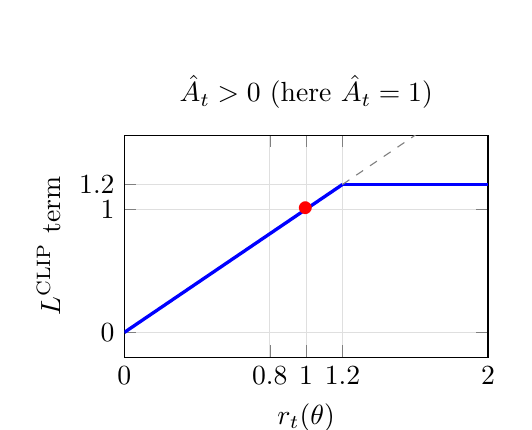
\begin{tikzpicture}
\begin{axis}[width=6.2cm,height=4.4cm,xmin=0,xmax=2,ymin=-0.2,ymax=1.6,
  xlabel={$r_t(\theta)$},ylabel={$L^{\mathrm{CLIP}}$ term},title={$\hA_t>0$ (here $\hA_t=1$)},
  xtick={0,0.8,1,1.2,2},ytick={0,1,1.2},grid=major,grid style={gray!25},
  every axis plot/.append style={very thick}]
  \addplot[blue,domain=0:1.2,samples=2]{x};
  \addplot[blue,domain=1.2:2,samples=2]{1.2};
  \addplot[gray,dashed,thin,domain=1.2:2,samples=2]{x};
  \node[red,font=\large] at (axis cs:1,1) {$\bullet$};
\end{axis}
\end{tikzpicture}
\hspace{0.8cm}
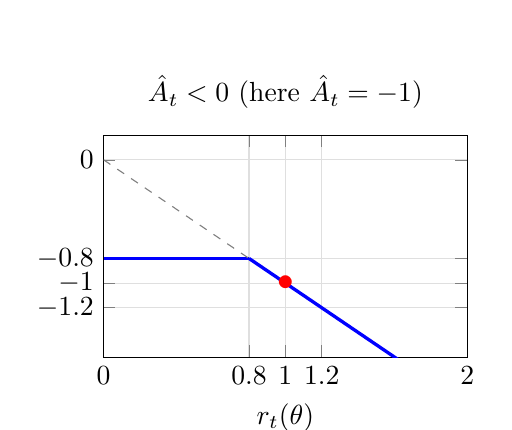
\begin{tikzpicture}
\begin{axis}[width=6.2cm,height=4.4cm,xmin=0,xmax=2,ymin=-1.6,ymax=0.2,
  xlabel={$r_t(\theta)$},title={$\hA_t<0$ (here $\hA_t=-1$)},
  xtick={0,0.8,1,1.2,2},ytick={-1.2,-1,-0.8,0},grid=major,grid style={gray!25},
  every axis plot/.append style={very thick}]
  \addplot[blue,domain=0:0.8,samples=2]{-0.8};
  \addplot[blue,domain=0.8:2,samples=2]{-x};
  \addplot[gray,dashed,thin,domain=0:0.8,samples=2]{-x};
  \node[red,font=\large] at (axis cs:1,-1) {$\bullet$};
\end{axis}
\end{tikzpicture}
\caption{One term of $L^{\mathrm{CLIP}}$ as a function of the ratio. The red dot is $r_t=1$, where every PPO update starts. Flat parts have zero gradient: once the ratio has moved $\varepsilon$ in the \enquote{good} direction, this sample stops pulling. In the \enquote{bad} direction there is no clipping, so mistakes are still corrected.}
\label{fig:clip}
\end{figure}

\paragraph{Case analysis} (see \cref{fig:clip}).
\begin{itemize}[nosep]
  \item $\hA_t>0$: we want to raise $\pi(a_t\mid s_t)$, i.e.\ increase $r_t$. The $\min$ caps the gain at $(1+\varepsilon)\hA_t$, so there is no incentive to push $r_t$ beyond $1+\varepsilon$.
  \item $\hA_t<0$: we want to lower $\pi(a_t\mid s_t)$. The gain is capped once $r_t<1-\varepsilon$.
  \item Because of the $\min$, the objective is a \emph{pessimistic} (lower) bound on the unclipped surrogate: clipping can only remove incentive, never add it.
\end{itemize}

\subsection{Implementation details that matter}
\begin{itemize}[nosep]
  \item \textbf{Computing the ratio.} Never divide probabilities; use log-probs:
        $r_t = \exp\big(\log\pit(a_t\mid s_t) - \log\pi_{\theta_{\mathrm{old}}}(a_t\mid s_t)\big)$.
        The new log-probs come from a fresh forward pass of the current network on \code{mb\_states}; the old ones are \code{mb\_old\_log\_probs}, stored detached during the rollout, so they are constants.
  \item \textbf{Several epochs over minibatches.} An \emph{epoch} is one pass over the whole rollout; a \emph{minibatch} is a random subset of it used for one gradient step. \code{update\_epochs}$=10$ passes over the 2048-step buffer in shuffled minibatches of 256, i.e.\ 80 gradient steps per rollout instead of 1. In the first minibatch $r_t\equiv1$; later minibatches see a policy that has already moved, and clipping becomes active.
  \item \textbf{Advantages} are the GAE values, standardised per rollout (already done in the notebook), so roughly half are positive and half negative and their scale does not depend on the reward scale.
  \item \textbf{Full loss.} PPO uses the same three-term structure as \eqref{eq:ac-loss}, but with the clipped policy term and the $\lambda$-returns as value targets:
\end{itemize}
\begin{keybox}{PPO loss (minimised)}
\vspace{-0.6em}
\begin{equation}
  L(\theta) = -\,\hat\E_t\Big[\min\big(r_t\hA_t,\ \clip(r_t,1-\varepsilon,1+\varepsilon)\hA_t\big)\Big]
  + c_V\,\hat\E_t\big[(V_\theta(s_t)-\hat R_t)^2\big]
  - c_H\,\hat\E_t\big[\Hent(\pit(\cdot\mid s_t))\big]
\end{equation}
$\hat\E_t$ is the mean over the minibatch; $\hat R_t$ = \code{mb\_returns}, $\hA_t$ = \code{mb\_advantages}.
\end{keybox}

\begin{todobox}{What you do in TODO 3 (PPO) and why}
\textbf{Goal.} For one minibatch of the rollout, produce one scalar \code{loss}: the PPO loss in the box above.

\textbf{Where you are in the loop.} A rollout of 2048 steps was collected with the policy as it was \emph{then} ($\theta_{\mathrm{old}}$), GAE advantages and $\lambda$-returns were computed, and the loop now runs 10 epochs over shuffled minibatches of 256. Since \code{optimizer.step()} runs after every minibatch, the network's current $\theta$ drifts away from $\theta_{\mathrm{old}}$ during these epochs. Unlike TODO 1--2, nothing from the current network has been computed yet: you must run the network yourself.

\begin{maptable}
$s_t$ & \code{mb\_states} & $(B,128)$ & \no & states from the rollout \\
$a_t$ & \code{mb\_actions} & $(B,)$ int & \no & actions taken in the rollout \\
$\log\pi_{\theta_{\mathrm{old}}}(a_t\mid s_t)$ & \code{mb\_old\_log\_probs} & $(B,)$ & \no & log-probs when the data was collected \\
$\hA_t$ & \code{mb\_advantages} & $(B,)$ & \no & GAE advantages (standardised) \\
$\hat R_t$ & \code{mb\_returns} & $(B,)$ & \no & $\lambda$-return targets for the critic \\
$\varepsilon$ & \code{clip\_range} & number & -- & how far the ratio may move ($0.2$) \\
\end{maptable}

\textbf{Steps.}
\begin{enumerate}[nosep]
  \item Run \code{net(mb\_states)}: logits $(B,6)$ and values $(B,)$, both with gradient.
  \item Build \code{Categorical(logits=...)}; get the new log-probs of \code{mb\_actions} $(B,)$ and the mean entropy.
  \item Ratio: \code{torch.exp(new\_log\_probs - mb\_old\_log\_probs)}.
  \item Two surrogates: ratio $\times$ advantages, and \code{torch.clamp}(ratio, $1-\varepsilon$, $1+\varepsilon$) $\times$ advantages.
  \item Policy term: minus the mean of the element-wise \code{torch.min} of the two.
  \item Value term: mean of \code{(values - mb\_returns)**2}; entropy term as in TODO 2.
  \item \code{loss} = policy term $+$ \code{value\_coef}$\cdot$value term $-$ \code{entropy\_coef}$\cdot$entropy.
\end{enumerate}

\textbf{How this is the theory.}
Steps 1--2 evaluate the \emph{current} policy $\pit$ on \emph{old} data, the situation importance sampling was made for (\cref{sec:onpolicy}).
Step 3 is the probability ratio $r_t(\theta)$ of the surrogate objective $L^{\mathrm{CPI}}$; the log-difference avoids dividing small probabilities.
Steps 4--5 are $L^{\mathrm{CLIP}}$: the $\min$ with the clipped version removes any incentive to move the ratio outside $[1-\varepsilon,1+\varepsilon]$ (\cref{fig:clip}), which is PPO's cheap replacement for TRPO's KL trust region. This is what makes 10 epochs on the same data safe.
Step 6 trains the critic on the GAE $\lambda$-returns (\cref{sec:gae}) instead of Monte Carlo returns. Step 7 is the same three-term structure as TODO 2.

\textbf{Sanity check.} In the first minibatch of every update the network has not changed yet, so the ratio is exactly 1 and both surrogates are equal.
\end{todobox}

\begin{pitfall}
\begin{itemize}[nosep,leftmargin=*]
  \item Using \code{torch.min} of the two terms, then forgetting the minus sign: you would \emph{minimise} the objective.
  \item Clipping the advantage instead of the ratio, or clipping $r_t\hA_t$ as a whole: wrong when $\hA_t<0$.
  \item Re-using the rollout's \code{log\_prob} (with gradient) instead of recomputing: the old log-probs must be constants and the new ones must come from the current parameters.
  \item Shape mismatch: values from \code{net(mb\_states)} have shape $(B,)$, matching \code{mb\_returns}. Avoid a $(B,1)$ tensor, which silently broadcasts to $(B,B)$ in the MSE.
\end{itemize}
\end{pitfall}

\paragraph{Data efficiency.} REINFORCE and A2C throw the data away after one gradient step (\cref{sec:onpolicy}). PPO is still on-policy, but the ratio (importance sampling) plus clipping lets it squeeze many gradient steps out of each rollout. This is why PPO, which is run for $10^6$ timesteps in A3, typically learns much faster per sample than the other two.

% ===========================================================================
\section{Continuous control: DPG and DDPG (TODO 4 and 5)}\label{sec:ddpg}

\subsection{Why a new method}
On Pendulum the action is a torque $a\in[-2,2]$. Options:
\begin{itemize}[nosep]
  \item Discretise it: loses precision, and the number of actions explodes with the action dimension.
  \item Stochastic Gaussian policy $\pit(a\mid s)=\mathcal N(\mu_\theta(s),\sigma^2)$ with the usual policy gradient: works (PPO does this for continuous control), but is on-policy.
  \item \textbf{Deterministic policy} $a=\mu_\theta(s)$ and differentiate the critic through the action: DDPG. This is \emph{Deep Q-learning for continuous actions}.
\end{itemize}
In DQN we act with $\argmax_a Q(s,a)$. For continuous $a$ we cannot enumerate actions, so we train a network $\mu_\theta(s)$ to \emph{approximate} that argmax by gradient ascent on $Q$.

\subsection{The deterministic policy gradient theorem}
For a deterministic policy, the objective is $J(\theta)=\E_{s\sim\rho^\mu}\big[Q^\mu(s,\mu_\theta(s))\big]$, where $\rho^\mu$ is the (discounted) \emph{state distribution}: how often each state is visited when acting with $\mu_\theta$. In words: \enquote{in the states we visit, the action we pick should have high $Q$.} Silver et al.\ (2014) show
\begin{equation}
  \gradt J(\theta) = \E_{s\sim\rho^\mu}\Big[\gradt\mu_\theta(s)\;\nabla_a Q^\mu(s,a)\big|_{a=\mu_\theta(s)}\Big].
  \label{eq:dpg}
\end{equation}
This is just the \textbf{chain rule}: $\frac{\partial Q(s,\mu_\theta(s))}{\partial\theta} = \frac{\partial\mu_\theta(s)}{\partial\theta}\cdot\frac{\partial Q(s,a)}{\partial a}$.
Intuition: the critic tells the actor \enquote{in state $s$, nudging the torque this way increases $Q$}; the actor follows that slope.
Compared with the stochastic policy gradient there is no $\log\pi$, no sampling over actions, and no expectation over $a$, so the variance is much lower.

\paragraph{Turning it into a loss.} Autograd applies the chain rule for us if we simply feed the actor's output into the critic:
\begin{equation}
  L_{\mathrm{actor}}(\theta) = -\frac1B\sum_{i=1}^B Q_w\big(s_i,\mu_\theta(s_i)\big).
\end{equation}
During \code{actor\_loss.backward()} the gradient flows from $Q$ back through the critic's layers into the action input, and from there into the actor's weights: exactly the two factors of the chain rule above.
Only $\theta$ is stepped (by \code{actor\_optimizer}); the critic is used as a fixed differentiable function here. Note that the actions in the loss are \emph{recomputed} by the current actor, not taken from the replay buffer (the buffer actions are old and noisy; we want to improve what the actor does \emph{now}).

\subsection{Training the critic: TD learning with target networks}
The critic $Q_w(s,a)$ is trained like DQN, but the \enquote{max over next actions} is replaced by the (target) actor's action, because the actor is our approximation of the $\argmax$.
\textbf{Target networks} are lagged copies of the actor and critic, $\mu_{\theta^-}$ and $Q_{w^-}$, with their own weights $\theta^-,w^-$. They are never trained by gradient descent; they only slowly follow the real networks and are used to compute the TD target.
\begin{keybox}{DDPG critic}
\vspace{-0.6em}
\begin{equation}
  y_i = r_i + \gamma\,(1-d_i)\,Q_{w^-}\big(s'_i,\ \mu_{\theta^-}(s'_i)\big),
  \qquad
  L_{\mathrm{critic}}(w) = \frac1B\sum_i\big(Q_w(s_i,a_i)-y_i\big)^2 .
\end{equation}
$w^-,\theta^-$ are the \emph{target} critic and actor (\code{critic\_target}, \code{actor\_target}); $a_i$ is the action from the buffer; $d_i$ is the done flag.
\end{keybox}
\begin{itemize}[nosep]
  \item \textbf{The target is a constant.} Compute $y_i$ inside \code{torch.no\_grad()} (or detach it). TD learning treats the target as a fixed label, like in supervised regression; letting gradients flow into it would also change the target to move towards the prediction, which is a different (and worse-behaved) algorithm.
  \item \textbf{Why target networks?} If the target were computed with the network being trained, every update of $w$ would also move the target, so the regression chases itself and can oscillate or diverge (same reason as in DQN). DDPG uses \emph{soft} updates, also called \textbf{Polyak averaging}: after every step, $w^-\gets\tau w+(1-\tau)w^-$ with $\tau=0.005$, i.e.\ the target keeps 99.5\% of its old weights and moves 0.5\% towards the current ones. This is already implemented at the end of the loop. DQN instead copied the weights every $C$ steps (a \enquote{hard} update).
  \item \textbf{The $(1-d_i)$ mask.} There is no future value after a terminal state.
\end{itemize}

\subsection{Why replay is allowed here}
A \textbf{replay buffer} stores past transitions $(s,a,r,s',d)$ (up to $10^6$ of them, oldest dropped first) and each update trains on a random minibatch from it. Random sampling breaks the strong correlation between consecutive steps, and each transition is reused many times.
This is only allowed because DDPG is \textbf{off-policy} (\cref{sec:onpolicy}): the critic update is a Bellman regression valid for any $(s,a,r,s')$, no matter which policy chose $a$, and the actor update \eqref{eq:dpg} has no expectation over actions, so no importance weights are needed. PPO/A2C cannot do this. The remaining mismatch is that states come from a mix of old policies rather than the current one; lecture 3.2 notes we simply accept this.

\paragraph{Exploration.} A deterministic policy always picks the same action in the same state, so it never tries alternatives. A3 therefore adds Gaussian noise to the action, $a=\clip(\mu_\theta(s)+\mathcal N(0,0.1^2),-2,2)$ (the continuous analogue of $\varepsilon$-greedy), and uses uniformly random actions for the first \code{start\_timesteps} steps (\emph{warm-up}) to fill the buffer with diverse data before the untrained actor is used. The noise is only used to collect data; the losses use the noise-free $\mu_\theta$.

\begin{algorithm}[H]
\caption{DDPG (one environment step), matching the A3 loop}
\begin{algorithmic}[1]
\State Act $a=\operatorname{clip}(\mu_\theta(s)+\text{noise})$, observe $r,s',d$; store $(s,a,r,s',d)$ in buffer $\mathcal D$
\State Sample minibatch $\{(s_i,a_i,r_i,s'_i,d_i)\}_{i=1}^B$ from $\mathcal D$
\State \textbf{Critic:} $y_i\gets r_i+\gamma(1-d_i)Q_{w^-}(s'_i,\mu_{\theta^-}(s'_i))$; \ step $w$ on $\frac1B\sum_i(Q_w(s_i,a_i)-y_i)^2$ \Comment{TODO 4}
\State \textbf{Actor:} step $\theta$ on $-\frac1B\sum_i Q_w(s_i,\mu_\theta(s_i))$ \Comment{TODO 5}
\State \textbf{Targets:} $w^-\gets\tau w+(1-\tau)w^-$, \ $\theta^-\gets\tau\theta+(1-\tau)\theta^-$
\end{algorithmic}
\end{algorithm}

\paragraph{Where you are in the loop (TODO 4 and 5).} After every environment step the loop samples a minibatch of $B=64$ old transitions from the replay buffer. TODO 4 updates the critic on it, TODO 5 then updates the actor, and afterwards the given code moves the target networks a little (Polyak). All five tensors from \code{replay\_buffer.sample} are plain data with no gradient.

\begin{todobox}{What you do in TODO 4 (DDPG critic) and why}
\textbf{Goal.} Compute the TD targets \code{target\_values} and the scalar \code{critic\_loss} from the \enquote{DDPG critic} box.

\begin{maptable}
$s_i,\ s'_i$ & \code{states}, \code{next\_states} & $(B,3)$ & \no & state before and after the step \\
$a_i$ & \code{actions} & $(B,1)$ & \no & action that was taken (with noise) \\
$r_i,\ d_i$ & \code{rewards}, \code{dones} & $(B,)$ & \no & reward and done flag (0 or 1) \\
$\mu_{\theta^-},\ Q_{w^-}$ & \code{actor\_target}, \code{critic\_target} & networks & \no & slow copies, used only for the target \\
$Q_w$ & \code{critic} & network & \yes & the network being trained \\
$y_i$ & \code{target\_values} & $(B,)$ & \no & what you must create \\
\end{maptable}

\textbf{Steps.}
\begin{enumerate}[nosep]
  \item Inside \code{with torch.no\_grad():} let the target actor choose next actions, $\mu_{\theta^-}(s'_i)$, shape $(B,1)$; evaluate them with the target critic, $Q_{w^-}(s'_i,\mu_{\theta^-}(s'_i))$, shape $(B,)$; then \code{target\_values} $= r_i+\gamma(1-d_i)\cdot$ that.
  \item Outside \code{no\_grad}: current estimates $Q_w(s_i,a_i)$ with the \emph{buffer} actions, shape $(B,)$.
  \item \code{critic\_loss} = mean squared difference between the two.
\end{enumerate}

\textbf{How this is the theory.}
Step 1 is the Bellman equation for a deterministic policy, $Q(s,a)=r+\gamma\,Q(s',\mu(s'))$: it is Q-learning's $r+\gamma\max_{a'}Q(s',a')$ with the $\max$ replaced by the actor, our approximation of the $\argmax$. Using the \emph{target} networks keeps the label from moving with every update; \code{no\_grad} makes it a fixed label (stop-gradient); $(1-d_i)$ removes the future value after a terminal state.
Step 2 uses the buffer action $a_i$ because we are asking \enquote{how good was the action that was actually taken?}, which is what the observed $r_i$ and $s'_i$ tell us about. This works for any old action, which is why replay is allowed (off-policy).
Step 3 is ordinary regression of $Q_w$ onto the labels.

\textbf{Sanity check.} \code{target\_values.shape == current\_q.shape == (B,)}, and \code{target\_values.requires\_grad} is \code{False}.
\end{todobox}

\begin{todobox}{What you do in TODO 5 (DDPG actor) and why}
\textbf{Goal.} Compute the scalar \code{actor\_loss} whose gradient moves the actor towards actions the critic rates higher.

\begin{maptable}
$s_i$ & \code{states} & $(B,3)$ & \no & same minibatch as TODO 4 \\
$\mu_\theta(s_i)$ & \code{actor(states)} & $(B,1)$ & \yes & what the actor would do \emph{now} \\
$Q_w(s_i,\mu_\theta(s_i))$ & \code{critic(states, ...)} & $(B,)$ & \yes & how good the critic thinks that is \\
\end{maptable}

\textbf{Steps.}
\begin{enumerate}[nosep]
  \item Let the current actor choose actions for \code{states} (no \code{no\_grad}: we need this gradient).
  \item Evaluate them with the current critic (not the target critic).
  \item \code{actor\_loss} = minus the mean of these $Q$-values.
\end{enumerate}

\textbf{How this is the theory.}
This is the deterministic policy gradient \eqref{eq:dpg}. Minimising $-Q$ is gradient ascent on $Q(s,\mu_\theta(s))$, and \code{backward()} applies the chain rule $\nabla_a Q\cdot\gradt\mu_\theta$ for you: the gradient flows from $Q$ through the critic's layers to the action input and on into the actor's weights. The critic is the \enquote{teacher} that tells the actor in which direction to change the torque. Fresh actor actions are used, not the buffer actions, because we want to improve what the actor does now. Only \code{actor\_optimizer.step()} follows, so the critic's weights are not changed by this loss.

\textbf{Sanity check.} As training goes on, $-$\code{actor\_loss} (the average $Q$) should rise and roughly track the (discounted) returns.
\end{todobox}

\begin{pitfall}
\begin{itemize}[nosep,leftmargin=*]
  \item \textbf{Shapes.} \code{DDPGCritic.forward} already squeezes to $(B,)$; \code{rewards} and \code{dones} from the buffer are $(B,)$. Keep everything $(B,)$. A $(B,1)$ vs.\ $(B,)$ mix broadcasts to $(B,B)$ and silently trains on garbage.
  \item \textbf{Actor loss uses the critic, not the target critic}, and the current actor $\mu_\theta(s_i)$, not the buffer action $a_i$.
  \item \textbf{Gradient leakage.} \code{actor\_loss.backward()} also writes gradients into the critic parameters. This is harmless here because \code{critic\_optimizer.zero\_grad()} clears them before the next critic step, and the actor optimiser only steps $\theta$.
  \item \textbf{Done vs.\ truncated.} Pendulum never terminates; episodes are only \emph{truncated} at 200 steps. The notebook stores \code{done = terminated or truncated}, so the last transition is treated as terminal. Theoretically one should bootstrap through a time-limit truncation (only \code{terminated} means \enquote{no future}); it is a small bias and you are not asked to change it.
\end{itemize}
\end{pitfall}

\subsection{Known weakness: overestimation, and TD3}
The critic's estimates contain random errors. As in Q-learning, maximising over noisy estimates is biased upwards ($\E[\max_i X_i]\ge\max_i\E[X_i]$): the actor actively seeks actions where the critic is \emph{wrongly} high, and the TD target copies that inflated value into other states. This systematic \textbf{overestimation} can make learning unstable. TD3 (lecture 3.4) adds three fixes: \emph{twin} critics with the minimum in the target (like double Q-learning), \emph{delayed} actor/target updates, and target policy smoothing (noise on $\mu_{\theta^-}(s')$). Not needed for A3, but useful if your DDPG curve is unstable.

% ===========================================================================
\section{Putting it together}\label{sec:summary}

\subsection{Cheat sheet}
\begin{center}
\begingroup
\renewcommand{\arraystretch}{1.35}
\small
\begin{tabularx}{\textwidth}{@{}l X l l@{}}
\toprule
Method & Policy term in the loss (minimised) & Critic target & Data \\
\midrule
REINFORCE & $-\hat\E_t[\log\pit(a_t\mid s_t)\,\tilde G_t]$ & none & on-policy \\
Actor-Critic & $-\hat\E_t[\log\pit(a_t\mid s_t)\,\operatorname{sg}(G_t-V(s_t))]$ & $G_t$ (MC) & on-policy \\
PPO & $-\hat\E_t[\min(r_t\hA_t,\clip(r_t,1\pm\varepsilon)\hA_t)]$ & $\hA^{\mathrm{GAE}}_t+V(s_t)$ & on-policy, $K$ epochs \\
DDPG & $-\hat\E_i[Q_w(s_i,\mu_\theta(s_i))]$ & $r+\gamma(1-d)\,Q_{w^-}(s',\mu_{\theta^-}(s'))$ & off-policy, replay \\
\bottomrule
\end{tabularx}
\endgroup
\end{center}
Here $\operatorname{sg}(\cdot)$ means stop-gradient (\code{.detach()}). Actor-critic and PPO additionally add $+\,c_V\cdot\text{MSE}(V,\text{target}) - c_H\cdot\text{entropy}$.

\subsection{What to expect when you run it}
\begin{itemize}[nosep]
  \item \textbf{Pong.} A random policy scores close to $-21$ (it loses every point). With the given budgets, REINFORCE and the episode-based actor-critic usually stay close to $-21$ or improve only slightly; PPO with $10^6$ steps should show a clearer upward trend. A curve that \emph{gets worse} from the start usually indicates a sign error.
  \item \textbf{Pendulum.} Returns per 200-step episode start around $-1200$ to $-1600$. A working DDPG typically climbs to roughly $-150$ to $-400$ within a few dozen episodes after the random warm-up.
  \item Results vary with the seed; the comparison in the plot is what matters for the report.
  \item \textbf{Quick checks:} all per-sample tensors 1-D with equal length; a minus on policy terms and the entropy bonus; constants (advantages, returns, old log-probs, TD targets) detached; PPO ratio exactly 1 in the first minibatch of each update.
\end{itemize}
\end{document}
